\documentclass{beamer}
%\documentclass[notes=only]{beamer}

\usepackage[utf8]{inputenc}
\usepackage{listings}
\usepackage{ulem}

\lstdefinestyle{customc}{
  belowcaptionskip=1\baselineskip,
  breaklines=true,
%  frame=L,
  xleftmargin=\parindent,
  language=C,
  showstringspaces=false,
  basicstyle=\scriptsize\ttfamily,
  keywordstyle=\bfseries\color{green!40!black},
  commentstyle=\itshape\color{purple!40!black},
  identifierstyle=\color{blue},
  stringstyle=\color{orange},
}
 
\usetheme{Dresden}

\title[SOFTENG 370 Tutorial 1 (2019)] %optional
{Linux, Pointers and pthreads}
  
\author{Edward Zhang}
 
% \institute[UoA] % (optional)
% {
%   Department of ECSE\\
%   The University of Auckland
% }
 
\date[July 2019] % (optional)
{SOFTENG 370 T1}

\begin{document}
\frame{\titlepage}
\begin{frame}
  \frametitle{Hello!}
  I'm in Part IV, and you probably remember me from SOFTENG 251, SOFTENG 206, and SOFTENG 254\\
  \begin{itemize}
    \item Ask questions on Piazza instead of emailing me so your classmates can see the answers (also such that Robert can answer questions that I can't, such as specifics regarding what you can and can't do in the assignment)
    \item If you want to meet, email me first at ezha210@aucklanduni.ac.nz
    \item These slides will be on Canvas, and any source code demonstrated along with TeX source code for these slides can be found on github.com/encryptededdy
  \end{itemize}
\end{frame}
\section{Running UNIX}
\begin{frame}
  \frametitle{You need a UNIX system}
  Some ways to get a UNIX system to do this assignment
  \begin{itemize}
    \item Dual Boot Linux
    \item Run Linux in a Virtual Machine
    \item Run natively on macOS
    \begin{itemize}
      \item Probably won't work for Assignment 2 (no FUSE)
    \end{itemize}
    \item \sout{Run within Windows Subsystem for Linux (WSL)}
    \begin{itemize}
      \item Stack size is fixed at 8192K - can only test around 0.5mil elements
    \end{itemize}
    \item Run within Windows Subsystem for Linux 2 (WSL2)
    \begin{itemize}
      \item Unreleased, unless you want to run Insider Fast Ring (not recommended)
    \end{itemize}
  \end{itemize}
\end{frame}
\begin{frame}
  \frametitle{On Virtual Machines}
  You can use any distro you want, but you'll probably be able to get more help when googling if you use one of the more popular desktop ones.
  \begin{itemize}
    \item Ubuntu (probably 18.04 LTS)
    \item Fedora Workstation (my personal preference)
    \item Debian
    \item Arch (great wiki, and u use arch btw), Manjaro if you actually want an installer
  \end{itemize}
\end{frame}
\begin{frame}
  \frametitle{Hypervisors}
  Oracle's VirtualBox is the usual free go-to. I personally prefer VMWare Player, feel free to give it a try. Parallels is a good option on macOS, but it's \$\$\$.\newline
  \newline
  Also try Hyper-V on Windows if you have Pro/Education (you can get Education for free using Azure dev tools for teaching) and already have it enabled, as it lets you keep other Windows features on (like Windows Sandbox or Core Isolation). It also supports one-click install of Ubuntu.
\end{frame}
\begin{frame}
  \frametitle{Note on Dual Booting}
    Beware you may be unable to dual-boot on some hardware, such as Surface Devices (drivers are a bit of a pain, especially on the book; check r/surfacelinux for more resources), or the 2019 MacBook Pro (can't even install, T2 chip NVMe storage support broken).
\end{frame}
\begin{frame}
  \frametitle{VSCode Remote}
  You can develop in a Linux environment with a Linux toolchain, while running VSCode from within Windows. This supports WSL and Linux systems over a SSH connection. Useful as it lets you run a headless VM while still being able to use VSCode to edit as if it was local.\\
  See: https://code.visualstudio.com/docs/remote/wsl
  % TODO: Add photos
\end{frame}
\begin{frame}
  \frametitle{Software to use}
  \begin{itemize}
    \item Install gcc (if not part of your distro) using apt/dnf/pacman
    \item Visual Studio Code is a fine text editor with IntelliSense
    \item You could also use CLion (JetBrains) if you prefer IntelliJ-like shortcuts and autocomplete, however you will need to create your own CMake file for building. There's no free version, but you can sign up for a JetBrains educational account
  \end{itemize}
\end{frame}
\section{Manpages}
\begin{frame}
  \frametitle{Using man to find documentation}
  \begin{columns}[c]
    \column{.5\textwidth}
      Man is a built in documentation tool. In this case, we can check the documentation for pthread\_create using\dots\\
      \texttt{\$ man pthread\_create}
    \column{.5\textwidth}
      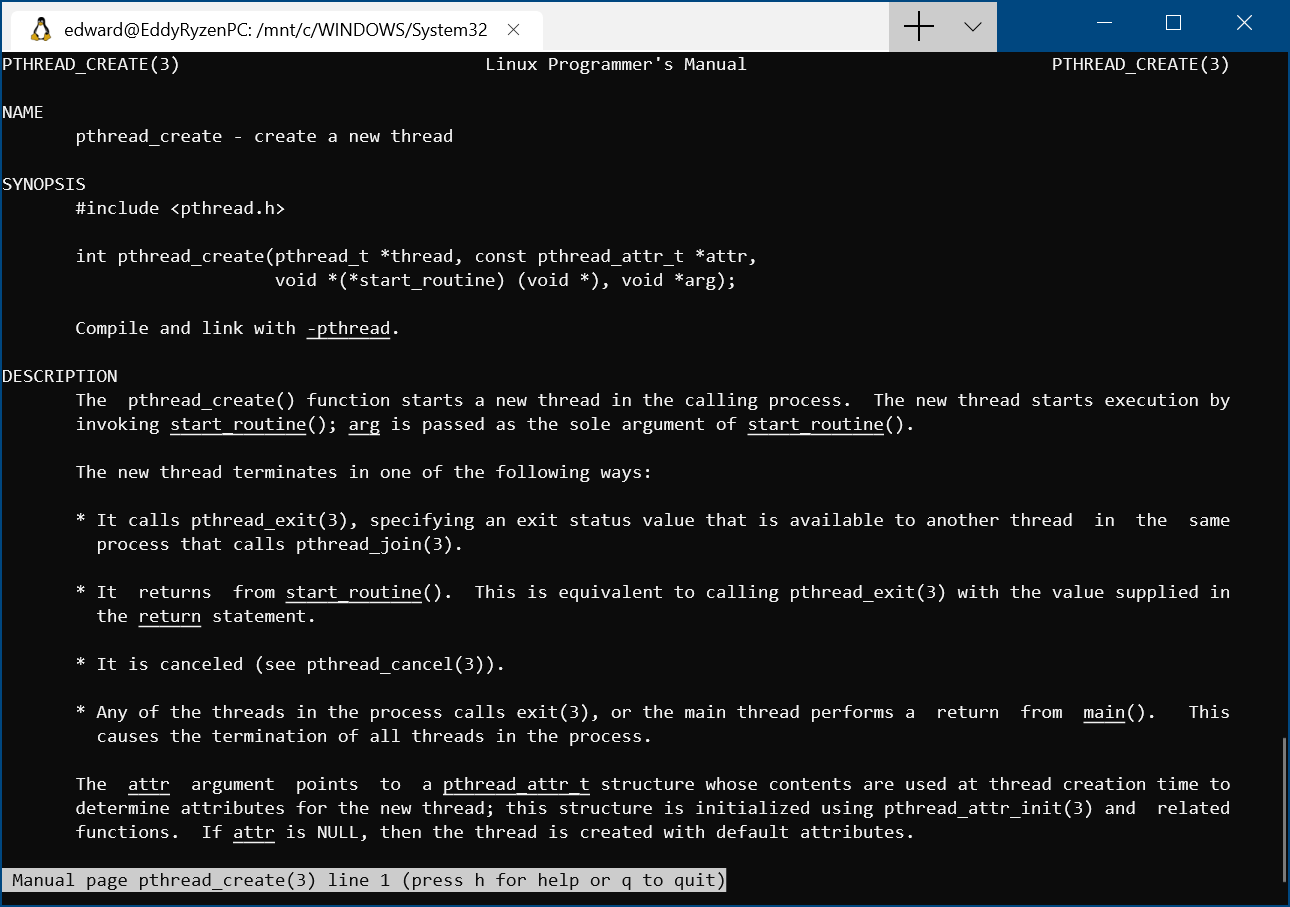
\includegraphics[width=\textwidth,height=\textheight,keepaspectratio]{pthreadmanpage.png}
  \end{columns}
\end{frame}
\begin{frame}
  \frametitle{Finding the correct manpage}
  \begin{columns}[c]
    \column{.5\textwidth}
      What if there are multiple versions of a given function?\\
      \texttt{\$ man 3 printf}\\
      Use 3 to access section 3, which contains the C function version of printf. Without 3 you get the linux command.
    \column{.5\textwidth}
      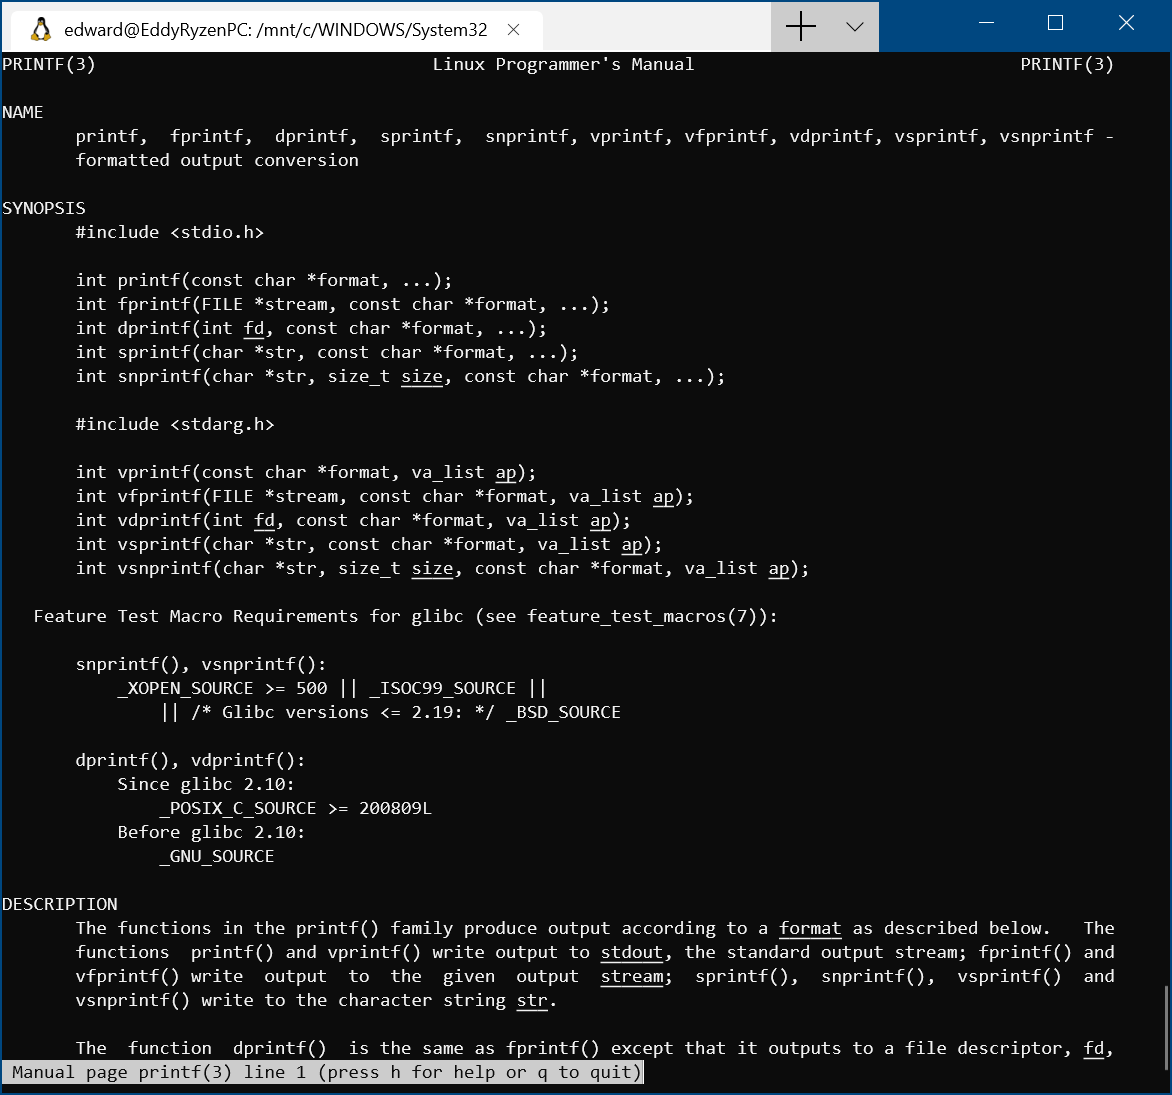
\includegraphics[width=\textwidth,height=\textheight,keepaspectratio]{manprintf.png}
  \end{columns}
\end{frame}
\section{Pointers}
\begin{frame}
  \frametitle{Defining Pointers}
  Consider a variable foo. Say we define it as \texttt{int foo;}
  \begin{itemize}
    \item \texttt{\&foo} gives us the address of foo.
    \item \texttt{int *fooPointer} stores a pointer to something of type int. Thus, we could do something like \texttt{int *fooPointer = \&foo;}
  \end{itemize}
\end{frame}
\begin{frame}
  \frametitle{Assignment / Dereferencing}
  Ok, now we have a pointer to foo that we defined with \texttt{int *fooPointer = \&foo;}. How can we write to what it's pointing too (foo)?
  \begin{itemize}
    \item You cannot just go \texttt{fooPointer = 12}
    \item We can instead dereference using an asterisk and perform a store, such as \texttt{*fooPointer = 12}
    \item We can load the value such as \texttt{int bar = *fooPointer;}
    \item Note that once we load it into bar, updating bar won't change foo.
  \end{itemize}
\end{frame}
\begin{frame}
  \frametitle{Example}
  \lstinputlisting[style=customc]{code/basicPointers.c}
\end{frame}
\begin{frame}[fragile]
  \frametitle{Indirection}
  You can do this by the way..
  \begin{lstlisting}[style=customc]
    int    a =  100;
    int   *b = &a;
    int  **c = &b;
    int ***d = &c;
  \end{lstlisting}
  And to dereference these, use the appropriate number of asterisks
  \begin{lstlisting}[style=customc]
    ***d == **c == *b == a == 100;
  \end{lstlisting}
  Note that **d would return a type int * (b), and *d would return a type int ** (c).
\end{frame}
\begin{frame}[fragile]
  \frametitle{Function Pointers}
  There are cases where we have to pass around functions, and for that we can use function pointers! Consider this function\dots
  \begin{lstlisting}[style=customc]
    void meme(int a) {
      printf("Nobody: 0, C: %d", a);
    }
  \end{lstlisting}
  To define a variable that stores a function that returns void and takes an int, then assign it with the meme function, we can do this\dots
  \begin{lstlisting}[style=customc]
    void (*funcPtr)(int);
    funcPtr = &meme;
  \end{lstlisting}
  In order to call funcPtr, we simply dereference it and give it the input we want.
  \begin{lstlisting}[style=customc]
    (*funcPtr)(370); // prints Nobody: 0, C: 370
  \end{lstlisting}
\end{frame}
\begin{frame}[fragile]
  \frametitle{Function Pointers cont.}
  This is useful if we want a function that takes a function as a parameter...
  \begin{lstlisting}[style=customc]
    void caller(void (*func)(int)) 
    { 
        func(100);
    } 
  \end{lstlisting}
  ...prehaps by a library that helps you run your function on a seperate thread :thinking:
\end{frame}
\begin{frame}[fragile]
  \frametitle{What's this?}
  Consider this section of code from the assignment. What's happening here?
  \begin{lstlisting}[style=customc]
  struct block right_block;
  struct block left_block;
  left_block.size = my_data->size / 2;
  left_block.first = my_data->first;
  right_block.size = left_block.size + (my_data->size % 2);
  right_block.first = my_data->first + left_block.size;
  merge_sort(&left_block);
  merge_sort(&right_block);
  merge(&left_block, &right_block);
  \end{lstlisting}
  Recall that the block struct has \texttt{size} as an int, and \texttt{first} as an *int
\end{frame}
\begin{frame}[fragile]
  \frametitle{Pointer Addition}
  If the first element is at memory location 0, then the second is at 4, then 8 and so on. (ints are usually 4 bytes).
  \begin{lstlisting}[style=customc]
  right_block.first = my_data->first + left_block.size;
  \end{lstlisting}
  When we add \texttt{size} to \texttt{first}, we essentially shift the pointer forward by \texttt{size} elements (therefore selecting the second half). Note that we aren't adding \texttt{size} bytes. Since \texttt{first} is an int pointer, (size of int $\times$ \texttt{size}) bytes are added.
\end{frame}
\section{Structures}
\begin{frame}[fragile] % Fragile needed for verbatim envs.
  \frametitle{Structure Basics}
  We can define a struct that holds multiple variables like this\dots
  \begin{lstlisting}[style=customc]
    struct Stuff
    {
      int a;
      int b;
    }
  \end{lstlisting}
  \pause
  And declare and assign to it\dots
  \begin{lstlisting}[style=customc]
    struct Stuff foo;
    foo.a = 0;
    foo.b = 1;
    // or
    struct Stuff foo = {0, 1};
  \end{lstlisting}
\end{frame}
\begin{frame}[fragile]
  \frametitle{Pointing to structs}
  \begin{lstlisting}[style=customc]
    struct Stuff foo = {0, 1};
    struct Stuff *fooPtr = &foo;
  \end{lstlisting}
  Now we have a pointer to a struct. But how do we access a and b inside it using the pointer?\\
  \pause
  Well, we could dereference it\dots
  \begin{lstlisting}[style=customc]
    (*fooPtr).a
    (*fooPtr).b
  \end{lstlisting}
  But that's ugly. So instead we can use an arrow (``pointer to member'')\dots
  \begin{lstlisting}[style=customc]
    fooPtr->a
    fooPtr->b
  \end{lstlisting}
\end{frame}
\section{Memory Allocation}
\begin{frame}[fragile]
  \frametitle{Lifetime of a stack variable}
  If we just initialize a variable like we do with ``local'' below, it is simply allocated on the stack. Recall that the stack is freed once a function returns.
  \begin{lstlisting}[style=customc]
  int* func()
  {
    int local = 7;
    return &local;
  }
  \end{lstlisting}
  What's wrong with this code?\\
  \pause
  A: After we return this function, local will be removed from the stack. Therefore, when whatever calls func tries to dereference the pointer that was returned, it may not point to what we want it to.
\end{frame}
\begin{frame}
  \frametitle{malloc}
  \begin{columns}[c]
    \column{.5\textwidth}
      Allocates a give number of bytes (not on the stack!), and return a pointer to said memory. We can then store stuff at this memory location that won't be lost when our function returns.
    \column{.5\textwidth}
      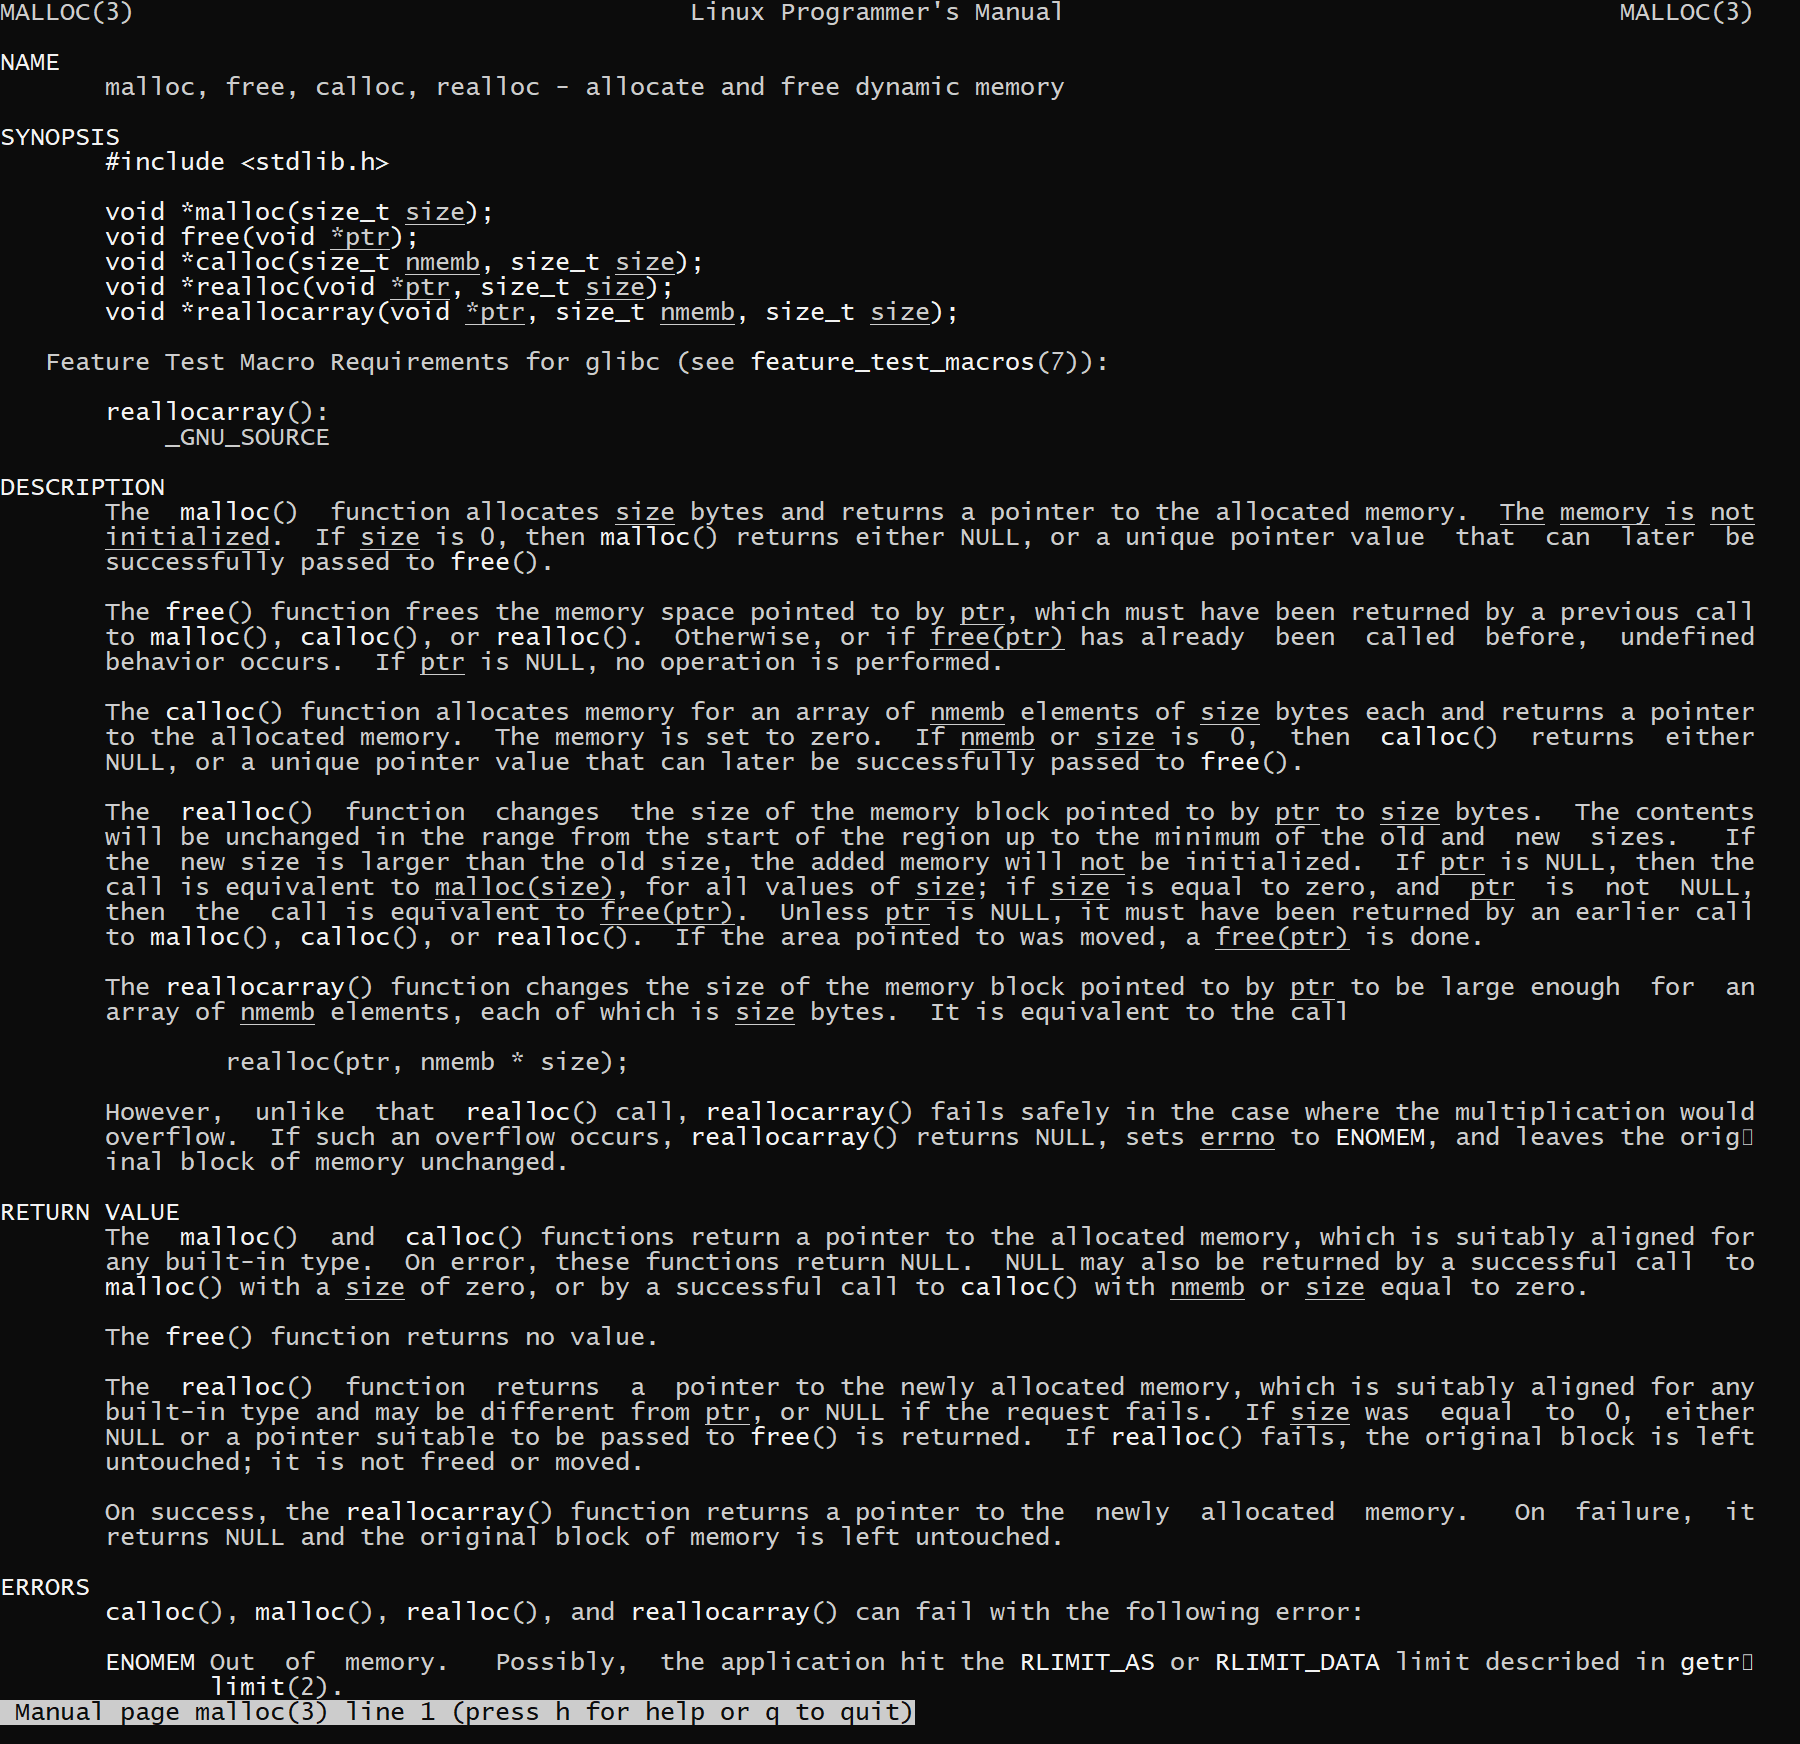
\includegraphics[width=\textwidth,height=\textheight,keepaspectratio]{manmalloc.png}
  \end{columns}
\end{frame}
\begin{frame}[fragile]
  \frametitle{Using malloc}
  Let's update our simple code from before to use malloc, such that we can safely return the poiner.
  \begin{lstlisting}[style=customc]
    int* func()
    {
      int *pointer;
      pointer = (int *)malloc(sizeof(int));
      if (pointer == 0)
      {
        // Couldn't malloc, probably out of memory
        return 0;
      }
      *pointer = 7
      return pointer;
    }
    \end{lstlisting}
\end{frame}
\begin{frame}
  \frametitle{More memory management}
  There way more to memory management than just using malloc, however you should look into this yourself.
  \begin{itemize}
    \item Use free(pointer) to free memory after you're doing using item
    \item Using malloc to create dynamically sized arrays (not strictly needed after C99) or other data structures
    \item Malloc does not initialize the memory to 0. Use \texttt{calloc} for that (slower)
    \item \texttt{realloc} to change the size of already malloc-ed memory
  \end{itemize}
  Use \texttt{man} to find out more!
\end{frame}
\section{pthreads}
\begin{frame}[fragile]
  \frametitle{pthread\_create}
  \begin{lstlisting}[style=customc]
    int pthread_create(
      pthread_t *thread, 
      const pthread_attr_t *attr, 
      void *(*start_routine) (void *), 
      void *arg
    );
  \end{lstlisting}
  \texttt{*thread}: Pointer to a \texttt{pthread\_t} struct at which a data about the thread will be stored.\\
  \pause
  \texttt{*attr}: A pointer to a \texttt{pthread\_attr\_t} struct with parameters for the thread. If you have no parameters to pass, you can set this to NULL.\\
  \pause
  \texttt{(*start\_routine)}: A function pointer to a function that takes one arg of type void* and has a return value of void*.\\
  \pause
  \texttt{*arg}: Pointer to the argument for the above function.
\end{frame}
\begin{frame}
  \frametitle{\texttt{void*} pointer?}
  A pointer to void is basically a ``generic'' pointer.
\end{frame}
\end{document}